% Options for packages loaded elsewhere
\PassOptionsToPackage{unicode}{hyperref}
\PassOptionsToPackage{hyphens}{url}
\PassOptionsToPackage{dvipsnames,svgnames,x11names}{xcolor}
%
\documentclass[
  letterpaper,
  DIV=11,
  numbers=noendperiod]{scrartcl}

\usepackage{amsmath,amssymb}
\usepackage{lmodern}
\usepackage{iftex}
\ifPDFTeX
  \usepackage[T1]{fontenc}
  \usepackage[utf8]{inputenc}
  \usepackage{textcomp} % provide euro and other symbols
\else % if luatex or xetex
  \usepackage{unicode-math}
  \defaultfontfeatures{Scale=MatchLowercase}
  \defaultfontfeatures[\rmfamily]{Ligatures=TeX,Scale=1}
\fi
% Use upquote if available, for straight quotes in verbatim environments
\IfFileExists{upquote.sty}{\usepackage{upquote}}{}
\IfFileExists{microtype.sty}{% use microtype if available
  \usepackage[]{microtype}
  \UseMicrotypeSet[protrusion]{basicmath} % disable protrusion for tt fonts
}{}
\makeatletter
\@ifundefined{KOMAClassName}{% if non-KOMA class
  \IfFileExists{parskip.sty}{%
    \usepackage{parskip}
  }{% else
    \setlength{\parindent}{0pt}
    \setlength{\parskip}{6pt plus 2pt minus 1pt}}
}{% if KOMA class
  \KOMAoptions{parskip=half}}
\makeatother
\usepackage{xcolor}
\setlength{\emergencystretch}{3em} % prevent overfull lines
\setcounter{secnumdepth}{-\maxdimen} % remove section numbering
% Make \paragraph and \subparagraph free-standing
\ifx\paragraph\undefined\else
  \let\oldparagraph\paragraph
  \renewcommand{\paragraph}[1]{\oldparagraph{#1}\mbox{}}
\fi
\ifx\subparagraph\undefined\else
  \let\oldsubparagraph\subparagraph
  \renewcommand{\subparagraph}[1]{\oldsubparagraph{#1}\mbox{}}
\fi

\usepackage{color}
\usepackage{fancyvrb}
\newcommand{\VerbBar}{|}
\newcommand{\VERB}{\Verb[commandchars=\\\{\}]}
\DefineVerbatimEnvironment{Highlighting}{Verbatim}{commandchars=\\\{\}}
% Add ',fontsize=\small' for more characters per line
\usepackage{framed}
\definecolor{shadecolor}{RGB}{46,52,64}
\newenvironment{Shaded}{\begin{snugshade}}{\end{snugshade}}
\newcommand{\AlertTok}[1]{\textcolor[rgb]{0.75,0.38,0.42}{\textbf{\colorbox[rgb]{0.23,0.26,0.32}{#1}}}}
\newcommand{\AnnotationTok}[1]{\textcolor[rgb]{0.82,0.53,0.44}{#1}}
\newcommand{\AttributeTok}[1]{\textcolor[rgb]{0.56,0.74,0.73}{#1}}
\newcommand{\BaseNTok}[1]{\textcolor[rgb]{0.71,0.56,0.68}{#1}}
\newcommand{\BuiltInTok}[1]{\textcolor[rgb]{0.53,0.75,0.82}{\textit{#1}}}
\newcommand{\CharTok}[1]{\textcolor[rgb]{0.92,0.80,0.55}{#1}}
\newcommand{\CommentTok}[1]{\textcolor[rgb]{0.38,0.43,0.53}{#1}}
\newcommand{\CommentVarTok}[1]{\textcolor[rgb]{0.90,0.91,0.94}{#1}}
\newcommand{\ConstantTok}[1]{\textcolor[rgb]{0.93,0.94,0.96}{\textbf{#1}}}
\newcommand{\ControlFlowTok}[1]{\textcolor[rgb]{0.51,0.63,0.76}{\textbf{#1}}}
\newcommand{\DataTypeTok}[1]{\textcolor[rgb]{0.51,0.63,0.76}{#1}}
\newcommand{\DecValTok}[1]{\textcolor[rgb]{0.71,0.56,0.68}{#1}}
\newcommand{\DocumentationTok}[1]{\textcolor[rgb]{0.37,0.51,0.67}{#1}}
\newcommand{\ErrorTok}[1]{\textcolor[rgb]{0.75,0.38,0.42}{\underline{#1}}}
\newcommand{\ExtensionTok}[1]{\textcolor[rgb]{0.56,0.74,0.73}{\textbf{#1}}}
\newcommand{\FloatTok}[1]{\textcolor[rgb]{0.71,0.56,0.68}{#1}}
\newcommand{\FunctionTok}[1]{\textcolor[rgb]{0.53,0.75,0.82}{#1}}
\newcommand{\ImportTok}[1]{\textcolor[rgb]{0.64,0.75,0.55}{#1}}
\newcommand{\InformationTok}[1]{\textcolor[rgb]{0.92,0.80,0.55}{#1}}
\newcommand{\KeywordTok}[1]{\textcolor[rgb]{0.51,0.63,0.76}{\textbf{#1}}}
\newcommand{\NormalTok}[1]{\textcolor[rgb]{0.85,0.87,0.91}{#1}}
\newcommand{\OperatorTok}[1]{\textcolor[rgb]{0.51,0.63,0.76}{#1}}
\newcommand{\OtherTok}[1]{\textcolor[rgb]{0.56,0.74,0.73}{#1}}
\newcommand{\PreprocessorTok}[1]{\textcolor[rgb]{0.37,0.51,0.67}{#1}}
\newcommand{\RegionMarkerTok}[1]{\textcolor[rgb]{0.53,0.75,0.82}{\colorbox[rgb]{0.23,0.26,0.32}{#1}}}
\newcommand{\SpecialCharTok}[1]{\textcolor[rgb]{0.92,0.80,0.55}{#1}}
\newcommand{\SpecialStringTok}[1]{\textcolor[rgb]{0.82,0.53,0.44}{#1}}
\newcommand{\StringTok}[1]{\textcolor[rgb]{0.64,0.75,0.55}{#1}}
\newcommand{\VariableTok}[1]{\textcolor[rgb]{0.37,0.51,0.67}{#1}}
\newcommand{\VerbatimStringTok}[1]{\textcolor[rgb]{0.64,0.75,0.55}{#1}}
\newcommand{\WarningTok}[1]{\textcolor[rgb]{0.75,0.38,0.42}{#1}}

\providecommand{\tightlist}{%
  \setlength{\itemsep}{0pt}\setlength{\parskip}{0pt}}\usepackage{longtable,booktabs,array}
\usepackage{calc} % for calculating minipage widths
% Correct order of tables after \paragraph or \subparagraph
\usepackage{etoolbox}
\makeatletter
\patchcmd\longtable{\par}{\if@noskipsec\mbox{}\fi\par}{}{}
\makeatother
% Allow footnotes in longtable head/foot
\IfFileExists{footnotehyper.sty}{\usepackage{footnotehyper}}{\usepackage{footnote}}
\makesavenoteenv{longtable}
\usepackage{graphicx}
\makeatletter
\def\maxwidth{\ifdim\Gin@nat@width>\linewidth\linewidth\else\Gin@nat@width\fi}
\def\maxheight{\ifdim\Gin@nat@height>\textheight\textheight\else\Gin@nat@height\fi}
\makeatother
% Scale images if necessary, so that they will not overflow the page
% margins by default, and it is still possible to overwrite the defaults
% using explicit options in \includegraphics[width, height, ...]{}
\setkeys{Gin}{width=\maxwidth,height=\maxheight,keepaspectratio}
% Set default figure placement to htbp
\makeatletter
\def\fps@figure{htbp}
\makeatother

\usepackage{booktabs}
\usepackage{longtable}
\usepackage{array}
\usepackage{multirow}
\usepackage{wrapfig}
\usepackage{float}
\usepackage{colortbl}
\usepackage{pdflscape}
\usepackage{tabu}
\usepackage{threeparttable}
\usepackage{threeparttablex}
\usepackage[normalem]{ulem}
\usepackage{makecell}
\usepackage{xcolor}
\usepackage{siunitx}
\newcolumntype{d}{S[input-symbols = ()]}
\usepackage{caption}
\usepackage{graphicx}
\usepackage{siunitx}
\usepackage{hhline}
\usepackage{calc}
\usepackage{tabularx}
\usepackage{adjustbox}
\usepackage{hyperref}
\KOMAoption{captions}{tableheading}
\makeatletter
\makeatother
\makeatletter
\makeatother
\makeatletter
\@ifpackageloaded{caption}{}{\usepackage{caption}}
\AtBeginDocument{%
\ifdefined\contentsname
  \renewcommand*\contentsname{Table of contents}
\else
  \newcommand\contentsname{Table of contents}
\fi
\ifdefined\listfigurename
  \renewcommand*\listfigurename{List of Figures}
\else
  \newcommand\listfigurename{List of Figures}
\fi
\ifdefined\listtablename
  \renewcommand*\listtablename{List of Tables}
\else
  \newcommand\listtablename{List of Tables}
\fi
\ifdefined\figurename
  \renewcommand*\figurename{Figure}
\else
  \newcommand\figurename{Figure}
\fi
\ifdefined\tablename
  \renewcommand*\tablename{Table}
\else
  \newcommand\tablename{Table}
\fi
}
\@ifpackageloaded{float}{}{\usepackage{float}}
\floatstyle{ruled}
\@ifundefined{c@chapter}{\newfloat{codelisting}{h}{lop}}{\newfloat{codelisting}{h}{lop}[chapter]}
\floatname{codelisting}{Listing}
\newcommand*\listoflistings{\listof{codelisting}{List of Listings}}
\makeatother
\makeatletter
\@ifpackageloaded{caption}{}{\usepackage{caption}}
\@ifpackageloaded{subcaption}{}{\usepackage{subcaption}}
\makeatother
\makeatletter
\makeatother
\ifLuaTeX
  \usepackage{selnolig}  % disable illegal ligatures
\fi
\IfFileExists{bookmark.sty}{\usepackage{bookmark}}{\usepackage{hyperref}}
\IfFileExists{xurl.sty}{\usepackage{xurl}}{} % add URL line breaks if available
\urlstyle{same} % disable monospaced font for URLs
\hypersetup{
  pdftitle={Linear Regression with Multiple Regressors},
  pdfauthor={Zahid Asghar   School of Economics, QAU, Islamabad},
  colorlinks=true,
  linkcolor={blue},
  filecolor={Maroon},
  citecolor={Blue},
  urlcolor={Blue},
  pdfcreator={LaTeX via pandoc}}

\title{Linear Regression with Multiple Regressors}
\author{Zahid Asghar School of Economics, QAU, Islamabad}
\date{}

\begin{document}
\maketitle
\hypertarget{outline}{%
\subsection{Outline}\label{outline}}

\begin{enumerate}
\def\labelenumi{\arabic{enumi}.}
\item
  Omitted variable bias
\item
  Causality and regression analysis
\item
  Multiple regression and OLS
\item
  Measures of fit\\
\item
  Sampling distribution of the OLS estimator
\end{enumerate}

\hypertarget{omitted-variable-bias}{%
\subsection{Omitted Variable Bias}\label{omitted-variable-bias}}

The error \(u\) arises because of factors, or variables, that influence
Y but are not included in the regression function. There are always
omitted variables. Sometimes, the omission of those variables can lead
to bias in the OLS estimator.

The bias in the OLS estimator that occurs as a result of an omitted
factor, or variable, is called omitted variable bias. For omitted
variable bias to occur, the omitted variable \(Z\) must satisfy two
conditions: The two conditions for omitted variable bias (1) \(Z\) is a
determinant of \(Y\) (i.e.~\(Z\) is part of \(u\)); and

(2) \(Z\) is correlated with the regressor \(X\)
i.e.~\(corr(Z,X) \neq 0\)

\textbf{Both} conditions must hold for the omission of \(Z\) to result
in omitted variable bias.

\hypertarget{section}{%
\subsection{}\label{section}}

\begin{itemize}
\item
  In the test score example:

  \begin{enumerate}
  \def\labelenumi{\arabic{enumi}.}
  \tightlist
  \item
    English language ability (whether the student has English as a
    second language) plausibly affects standardized test scores: \(Z\)
    is a determinant of \(Y\).
  \item
    Immigrant communities tend to be less affluent and thus have smaller
    school budgets and higher STR: \(Z\) is correlated with \$X\$.
    Accordingly, \(\hat\beta_1\) is biased. What is the direction of
    this bias?
  \end{enumerate}
\item
  What does common sense suggest?
\item
  If common sense fails you, there is a
  formula\ldots{}\(\sum^n_{i = 1} (Y_i - b_0 - b_1 X_i)^2\).
\end{itemize}

\[\begin{align}
{\hat\beta_1}-\beta_1 = \frac{1}{n} \frac{\sum^n_{i = 1}  \left(X_i - \bar{X} \right) u_i  }  {\sum^n_{i = 1}(X_i - \bar{X})^2}. \tag{6.1}
\end{align}\]

\hypertarget{section-1}{%
\subsection{}\label{section-1}}

From \(E(u_i\vert X_i) = 0\) implies \(corr(X_i,u_i)=0\)

\[\hat\beta_1 \xrightarrow[]{p} \beta_1 + \rho_{Xu} \frac{\sigma_u}{\sigma_X}. \tag{6.1}\]

\begin{itemize}
\item
  If If an omitted variable \(Z\) is both: (1) a determinant of \(Y\)
  (that is, it is contained in \(u\)); and (2) correlated with \(X\),
  then \(\rho_{Xu} \neq0\), and the OLS estimator \(\hat{\beta_1}\) is
  biased and is not consistent.
\item
  For example, districts with few ESL students (1) do better on
  standardized tests and (2) have smaller classes (bigger budgets), so
  ignoring the effect of having many ESL students factor would result in
  overstating the class size effect. Is this is actually going on in the
  CA data?
\end{itemize}

\hypertarget{table-6.1}{%
\subsection{Table 6.1}\label{table-6.1}}

\begin{Shaded}
\begin{Highlighting}[]
\FunctionTok{library}\NormalTok{(haven)}
\FunctionTok{library}\NormalTok{(kableExtra)}
\FunctionTok{library}\NormalTok{(tidyverse)}
\end{Highlighting}
\end{Shaded}

\begin{verbatim}
-- Attaching packages --------------------------------------- tidyverse 1.3.2 --
v ggplot2 3.3.6     v purrr   0.3.4
v tibble  3.1.7     v dplyr   1.0.9
v tidyr   1.2.0     v stringr 1.4.0
v readr   2.1.2     v forcats 0.5.1
-- Conflicts ------------------------------------------ tidyverse_conflicts() --
x dplyr::filter()     masks stats::filter()
x dplyr::group_rows() masks kableExtra::group_rows()
x dplyr::lag()        masks stats::lag()
\end{verbatim}

\begin{Shaded}
\begin{Highlighting}[]
\NormalTok{caschool }\OtherTok{\textless{}{-}} \FunctionTok{read\_dta}\NormalTok{(}\StringTok{"caschool.dta"}\NormalTok{)}
\FunctionTok{library}\NormalTok{(modelsummary)}
\FunctionTok{library}\NormalTok{(rstatix)}
\end{Highlighting}
\end{Shaded}

\begin{verbatim}

Attaching package: 'rstatix'

The following object is masked from 'package:stats':

    filter
\end{verbatim}

\begin{Shaded}
\begin{Highlighting}[]
\NormalTok{caschool}\OtherTok{\textless{}{-}}\NormalTok{caschool }\SpecialCharTok{\%\textgreater{}\%} \FunctionTok{mutate}\NormalTok{(}\AttributeTok{elq1=}\FunctionTok{ifelse}\NormalTok{(el\_pct}\SpecialCharTok{\textless{}=}\FloatTok{1.9}\NormalTok{,}\DecValTok{1}\NormalTok{,}\DecValTok{0}\NormalTok{))}
\NormalTok{caschool}\OtherTok{\textless{}{-}}\NormalTok{caschool }\SpecialCharTok{\%\textgreater{}\%} \FunctionTok{mutate}\NormalTok{(}\AttributeTok{elq2=}\FunctionTok{ifelse}\NormalTok{(el\_pct}\SpecialCharTok{\textgreater{}=}\FloatTok{1.9} \SpecialCharTok{\&}\NormalTok{ el\_pct}\SpecialCharTok{\textless{}}\FloatTok{8.8}\NormalTok{,}\DecValTok{1}\NormalTok{,}\DecValTok{0}\NormalTok{))}
\NormalTok{caschool}\OtherTok{\textless{}{-}}\NormalTok{caschool }\SpecialCharTok{\%\textgreater{}\%} \FunctionTok{mutate}\NormalTok{(}\AttributeTok{elq3=}\FunctionTok{ifelse}\NormalTok{(el\_pct}\SpecialCharTok{\textgreater{}=}\FloatTok{8.8} \SpecialCharTok{\&}\NormalTok{ el\_pct}\SpecialCharTok{\textless{}}\DecValTok{23}\NormalTok{,}\DecValTok{1}\NormalTok{,}\DecValTok{0}\NormalTok{))}
\NormalTok{caschool}\OtherTok{\textless{}{-}}\NormalTok{caschool }\SpecialCharTok{\%\textgreater{}\%} \FunctionTok{mutate}\NormalTok{(}\AttributeTok{elq4=}\FunctionTok{ifelse}\NormalTok{(el\_pct}\SpecialCharTok{\textgreater{}=}\DecValTok{23}\NormalTok{,}\DecValTok{1}\NormalTok{,}\DecValTok{0}\NormalTok{))}
\NormalTok{caschool}\OtherTok{\textless{}{-}}\NormalTok{caschool }\SpecialCharTok{\%\textgreater{}\%}   \FunctionTok{mutate}\NormalTok{(}\AttributeTok{str\_20 =} \FunctionTok{ifelse}\NormalTok{(str}\SpecialCharTok{\textless{}}\DecValTok{20}\NormalTok{, }\DecValTok{1}\NormalTok{,}\DecValTok{0}\NormalTok{))}
\end{Highlighting}
\end{Shaded}

\begin{Shaded}
\begin{Highlighting}[]
\NormalTok{overall}\OtherTok{\textless{}{-}}\NormalTok{caschool }\SpecialCharTok{\%\textgreater{}\%} \FunctionTok{t\_test}\NormalTok{(testscr}\SpecialCharTok{\textasciitilde{}}\NormalTok{str\_20,}\AttributeTok{var.equal=}\NormalTok{T)}
\NormalTok{el\_1}\FloatTok{.9}\OtherTok{\textless{}{-}}\NormalTok{caschool }\SpecialCharTok{\%\textgreater{}\%} \FunctionTok{filter}\NormalTok{(elq1}\SpecialCharTok{==}\DecValTok{1}\NormalTok{) }\SpecialCharTok{\%\textgreater{}\%} \FunctionTok{t\_test}\NormalTok{(testscr}\SpecialCharTok{\textasciitilde{}}\NormalTok{str\_20,}\AttributeTok{var.equal=}\NormalTok{T)}
\NormalTok{el\_8}\FloatTok{.8}\OtherTok{\textless{}{-}}\NormalTok{caschool }\SpecialCharTok{\%\textgreater{}\%} \FunctionTok{filter}\NormalTok{(elq2}\SpecialCharTok{==}\DecValTok{1}\NormalTok{) }\SpecialCharTok{\%\textgreater{}\%} \FunctionTok{t\_test}\NormalTok{(testscr}\SpecialCharTok{\textasciitilde{}}\NormalTok{str\_20,}\AttributeTok{var.equal=}\NormalTok{T)}
\NormalTok{el\_23}\OtherTok{\textless{}{-}}\NormalTok{caschool }\SpecialCharTok{\%\textgreater{}\%} \FunctionTok{filter}\NormalTok{(elq3}\SpecialCharTok{==}\DecValTok{1}\NormalTok{) }\SpecialCharTok{\%\textgreater{}\%} \FunctionTok{t\_test}\NormalTok{(testscr}\SpecialCharTok{\textasciitilde{}}\NormalTok{str\_20,}\AttributeTok{var.equal=}\NormalTok{T)}
\NormalTok{el\_gr23}\OtherTok{\textless{}{-}}\NormalTok{caschool }\SpecialCharTok{\%\textgreater{}\%} \FunctionTok{filter}\NormalTok{(elq4}\SpecialCharTok{==}\DecValTok{1}\NormalTok{) }\SpecialCharTok{\%\textgreater{}\%} \FunctionTok{t\_test}\NormalTok{(testscr}\SpecialCharTok{\textasciitilde{}}\NormalTok{str\_20,}\AttributeTok{var.equal=}\NormalTok{T)}
\NormalTok{table\_6}\FloatTok{.1}\OtherTok{\textless{}{-}}\FunctionTok{bind\_rows}\NormalTok{(overall,el\_1}\FloatTok{.9}\NormalTok{,el\_8}\FloatTok{.8}\NormalTok{,el\_23,el\_gr23)}

\NormalTok{df\_tbl}\OtherTok{\textless{}{-}} \FunctionTok{as\_tibble}\NormalTok{(table\_6}\FloatTok{.1}\NormalTok{)}
\NormalTok{df\_tbl}\OtherTok{\textless{}{-}}\NormalTok{df\_tbl }\SpecialCharTok{\%\textgreater{}\%} \FunctionTok{select}\NormalTok{(}\SpecialCharTok{{-}}\StringTok{".y."}\NormalTok{)}
\NormalTok{df\_tbl}\SpecialCharTok{$}\NormalTok{statistic}\OtherTok{\textless{}{-}}\FunctionTok{round}\NormalTok{(df\_tbl}\SpecialCharTok{$}\NormalTok{statistic,}\DecValTok{2}\NormalTok{)}
\NormalTok{df\_tbl}\SpecialCharTok{$}\NormalTok{p}\OtherTok{\textless{}{-}}\FunctionTok{round}\NormalTok{(df\_tbl}\SpecialCharTok{$}\NormalTok{p,}\DecValTok{3}\NormalTok{)}
\NormalTok{df\_tbl }
\end{Highlighting}
\end{Shaded}

\begin{verbatim}
# A tibble: 5 x 7
  group1 group2    n1    n2 statistic    df     p
  <chr>  <chr>  <int> <int>     <dbl> <dbl> <dbl>
1 0      1        182   238     -4      418 0    
2 0      1         27    76      0.27   101 0.789
3 0      1         44    64     -1.05   106 0.296
4 0      1         50    54     -1.73   102 0.087
5 0      1         61    44     -0.7    103 0.483
\end{verbatim}

\hypertarget{section-2}{%
\subsection{}\label{section-2}}

\begin{itemize}
\item
  Districts with fewer English Learners have higher test scores
\item
  Districts with lower percent EL (PctEL) have smaller classes
\item
  Among districts with comparable PctEL, the effect of class size
\end{itemize}

is small (recall overall ``test score gap'' = 7.4)

\hypertarget{section-3}{%
\subsection{}\label{section-3}}

Causality and regression analysis

The test score/STR/fraction English Learners example shows that, if an
omitted variable satisfies the two conditions for omitted variable bias,
then the OLS estimator in the regression omitting that variable is
biased and inconsistent. So, even if n is large, \(\hat{\beta_1}\) will
not be close to \(\beta_1\) . This raises a deeper question: how do we
define \(\beta_1\) ? That is, what precisely do we want to estimate when
we run a regression?

\hypertarget{section-4}{%
\subsection{}\label{section-4}}

What precisely do we want to estimate when we run a regression? There
are (at least) three possible answers to this question:

\begin{enumerate}
\def\labelenumi{\arabic{enumi}.}
\tightlist
\item
  We want to estimate the slope of a line through a scatterplot as a
  simple summary of the data to which we attach no substantive meaning.
  This can be useful at times, but isn't very interesting intellectually
  and isn't what this course is about.
\end{enumerate}

\hypertarget{section-5}{%
\subsection{}\label{section-5}}

\begin{enumerate}
\def\labelenumi{\arabic{enumi}.}
\setcounter{enumi}{1}
\tightlist
\item
  We want to make forecasts, or predictions, of the value of \(Y\) for
  an entity not in the data set, for which we know the value of \(X\).
\end{enumerate}

Forecasting is an important job for economists, and excellent forecasts
are possible using regression methods without needing to know causal
effects. We will return to forecasting later in the course.

\hypertarget{section-6}{%
\subsection{}\label{section-6}}

\begin{enumerate}
\def\labelenumi{\arabic{enumi}.}
\setcounter{enumi}{2}
\item
  We want to estimate the causal effect on Y of a change in \(X\).

  \emph{This is why we are interested in the class size effect. Suppose
  the school board decided to cut class size by 2 students per class.
  What would be the effect on test scores? This is a causal question
  (what is the causal effect on test scores of STR?) so we need to
  estimate this causal effect. Except when we discuss forecasting, the
  aim of this course is the estimation of causal effects using
  regression methods.}
\end{enumerate}

\hypertarget{what-precisely-is-a-causal-effect}{%
\subsection{What, precisely, is a causal
effect?}\label{what-precisely-is-a-causal-effect}}

\begin{itemize}
\tightlist
\item
  ``Causality'' is a complex concept!
\item
  In this course, we take a practical approach to defining causality:

  \begin{itemize}
  \tightlist
  \item
    \emph{A causal effect is defined to be the effect measure in an
    ideal randomized controlled experiment} \emph{in an ideal randomized
    controlled experiment.}
  \end{itemize}
\end{itemize}

\hypertarget{ideal-randomized-controlled-experiment}{%
\subsection{Ideal Randomized Controlled
Experiment}\label{ideal-randomized-controlled-experiment}}

\begin{itemize}
\tightlist
\item
  Ideal: subjects all follow the treatment protocol -- perfect
  compliance, no errors in reporting, etc.!
\item
  Randomized: subjects from the population of interest are randomly
  assigned to a treatment or control group (so there are no confounding
  factors)
\item
  Controlled: having a control group permits measuring the differential
  effect of the treatment
\item
  Experiment: the treatment is assigned as part of the experiment: the
  subjects have no choice, so there is no ``reverse causality'' in which
  subjects choose the treatment they think will work best.
\end{itemize}

\hypertarget{back-to-class-size}{%
\subsection{Back to class size:}\label{back-to-class-size}}

Imagine an ideal randomized controlled experiment for measuring the
effect on Test Score of reducing STR\ldots{}

\begin{itemize}
\item
  In that experiment, students would be randomly assigned to classes,
  which would have different sizes.
\item
  Because they are randomly assigned, all student characteristics (and
  thus \(u_i\)) would be distributed independently of STRi.
\item
  Thus, \(E(u_i|STR_i)=0\) -- that is, LSA \#1 holds in a randomized
  controlled experiment.
\end{itemize}

\hypertarget{section-7}{%
\subsection{}\label{section-7}}

How does our observational data differ from this ideal?

\begin{itemize}
\item
  The treatment is not randomly assigned
\item
  Consider PctEL -- percent English learners -- in the district.
\end{itemize}

It plausibly satisfies the two criteria for omitted variable bias: Z =
PctEL is:

\begin{enumerate}
\def\labelenumi{(\arabic{enumi})}
\item
  a determinant of Y; and
\item
  correlated with the regressor X.
\end{enumerate}

\begin{itemize}
\tightlist
\item
  Thus, the ``control'' and ``treatment'' groups differ in a systematic
  way, so \(corr(STR,PctEL)\neq0\)
\end{itemize}

\hypertarget{section-8}{%
\subsection{}\label{section-8}}

Randomization + control group means that any differences between the
treatment and control groups are random -- not systematically related to
the treatment

\begin{itemize}
\item
  We can eliminate the difference in PctEL between the large (control)
  and small (treatment) groups by examining the effect of class size
  among districts with the same PctEL.

  \begin{itemize}
  \item
    If the only systematic difference between the large and small class
    size groups is in PctEL, then we are back to the randomized
    controlled experiment -- within each PctEL group.
  \item
    This is one way to ``control'' for the effect of PctEL when
    estimating the effect of STR.
  \end{itemize}
\end{itemize}

\hypertarget{return-to-omitted-variable-bias}{%
\subsection{Return to omitted variable
bias}\label{return-to-omitted-variable-bias}}

Three ways to overcome omitted variable bias

\begin{enumerate}
\def\labelenumi{\arabic{enumi}.}
\item
  Run a randomized controlled experiment in which treatment (STR) is
  randomly assigned: then PctEL is still a determinant of TestScore, but
  PctEL is uncorrelated with STR. (This solution to OV bias is rarely
  feasible.)
\item
  Adopt the ``cross tabulation'' approach, with finer gradations of STR
  and PctEL -- within each group, all classes have the same PctEL, so we
  control for PctEL (But soon you will run out of data, and what about
  other determinants like family income and parental education?)
\item
  Use a regression in which the omitted variable (PctEL) is no longer
  omitted: include PctEL as an additional regressor in a multiple
  regression.
\end{enumerate}

\hypertarget{the-population-regression-function}{%
\subsection{The Population Regression
Function}\label{the-population-regression-function}}

Consider the two regressors:

\(Y_i = \beta_0 + \beta_1 X_{1i} + \beta_2 X_{2i} + u_i, \ i=1,\dots,n.\)

\begin{itemize}
\item
  \(Y_i\) is dependent variable
\item
  \(X1\), \(X2\) are the two independent variables (regressors)
\item
  (\(Y_i\), \(X_{1i}\), \(X_{2i}\)) denote the ith observation on \(Y\),
  \(X1\), and \(X2\).
\item
  \(\beta_0\) = unknown population intercept
\item
  \(\beta_1\) = effect on Y of a change in X1, holding X2 constant
\item
  \(\beta_2\) = effect on Y of a change in X2, holding X1 constant
\item
  \(u_i\) = the regression error (omitted factors)
\end{itemize}

\hypertarget{interpretation-of-coefficients-in-multiple-regression}{%
\subsection{Interpretation of coefficients in multiple
regression}\label{interpretation-of-coefficients-in-multiple-regression}}

\(Y_i = \beta_0 + \beta_1 X_{1i} + \beta_2 X_{2i} + u_i, \ i=1,\dots,n.\)\\
Consider changing \(X_1\) by \(X_1\) while holding \(X_2\) constant:
Population regression line \textbf{before} the change:
\(Y_i = \beta_0 + \beta_1 X_1 + \beta_2 X_2\)\\
Population regression line, after the change:
\(Y_i+{\Delta Y} = \beta_0 + \beta_1 (X_1+{\Delta X_1}) + \beta_2 X_2\)\\
Difference \textbf{After minus Before}
\({\Delta Y} = \beta_1 {\Delta X_1}\)

\(\beta_1=\frac{\Delta Y}{\Delta X_1}\) \textbf{holding} \(X_2\)
constant

\(\beta_2=\frac{\Delta Y}{\Delta X_2}\) \textbf{holding} \(X_1\)
constant

\(\beta_0 = predicted value of Y when X1 = X2 = 0\). (Theoretically
speaking)

\hypertarget{the-ols-estimator-in-multiple-regression}{%
\subsection{The OLS Estimator in Multiple
Regression}\label{the-ols-estimator-in-multiple-regression}}

(SW Section 6.3) With two regressors, the OLS estimator solves:
\(min_{b_1,b_2}\sum^n_{i = 1} (Y_i - b_0 - b_1 X_{1i}-b_2 X_{2i})^2.\)

\begin{itemize}
\item
  The OLS estimator minimizes the average squared difference between the
  actual values of Yi and the prediction (predicted value) based on the
  estimated line.
\item
  This minimization problem is solved using calculus
\item
  This yields the OLS estimators of \(\beta_0\) , \(\beta_1\) and
  \(\beta_2\)
\end{itemize}

\hypertarget{example-the-california-test-score-data}{%
\subsection{Example: the California test score
data}\label{example-the-california-test-score-data}}

Regression of TestScore against STR:

\(\widehat{TestScore}= 698.9 – 2.28STR\)

Now include percent English Learners in the district (PctEL):

\hypertarget{section-9}{%
\subsection{}\label{section-9}}

\begin{Shaded}
\begin{Highlighting}[]
\NormalTok{models}\OtherTok{\textless{}{-}}\FunctionTok{list}\NormalTok{(mod1}\OtherTok{\textless{}{-}}\FunctionTok{lm}\NormalTok{(testscr}\SpecialCharTok{\textasciitilde{}}\NormalTok{str,}\AttributeTok{data =}\NormalTok{ caschool),}
\NormalTok{mod2}\OtherTok{\textless{}{-}}\FunctionTok{lm}\NormalTok{(testscr}\SpecialCharTok{\textasciitilde{}}\NormalTok{str}\SpecialCharTok{+}\NormalTok{el\_pct,}\AttributeTok{data =}\NormalTok{ caschool))}
\NormalTok{mod1}\OtherTok{\textless{}{-}}\FunctionTok{lm}\NormalTok{(testscr}\SpecialCharTok{\textasciitilde{}}\NormalTok{str,}\AttributeTok{data =}\NormalTok{ caschool)}
\NormalTok{mod2}\OtherTok{\textless{}{-}}\FunctionTok{lm}\NormalTok{(testscr}\SpecialCharTok{\textasciitilde{}}\NormalTok{str}\SpecialCharTok{+}\NormalTok{el\_pct,}\AttributeTok{data =}\NormalTok{ caschool)}
\FunctionTok{modelsummary}\NormalTok{(}
\NormalTok{  models,}
  \AttributeTok{fmt =} \DecValTok{2}\NormalTok{,}
  \AttributeTok{estimate  =} \FunctionTok{c}\NormalTok{(}
                \StringTok{"\{estimate\} (\{std.error\})\{stars\}"}\NormalTok{),}
  \AttributeTok{statistic =} \ConstantTok{NULL}\NormalTok{)}
\end{Highlighting}
\end{Shaded}

\begin{table}
\centering
\begin{tabular}[t]{lcc}
\toprule
  & Model 1 & Model 2\\
\midrule
(Intercept) & \num{698.93} (\num{9.47})*** & \num{686.03} (\num{7.41})***\\
str & \num{-2.28} (\num{0.48})*** & \num{-1.10} (\num{0.38})**\\
el\_pct &  & \num{-0.65} (\num{0.04})***\\
\midrule
Num.Obs. & \num{420} & \num{420}\\
R2 & \num{0.051} & \num{0.426}\\
R2 Adj. & \num{0.049} & \num{0.424}\\
AIC & \num{3650.5} & \num{3441.1}\\
BIC & \num{3662.6} & \num{3457.3}\\
Log.Lik. & \num{-1822.250} & \num{-1716.561}\\
F & \num{22.575} & \num{155.014}\\
RMSE & \num{18.54} & \num{14.41}\\
\bottomrule
\end{tabular}
\end{table}

\hypertarget{section-10}{%
\subsection{}\label{section-10}}

\(\widehat{TestScore} = 686.0 – 1.10STR – 0.65PctEL\)

What happens to the coefficient on STR? - Why? (Note:
\(corr(STR, PctEL) = 0.19\))

Regression of TestScore against STR: TestScore

\hypertarget{section-11}{%
\subsection{}\label{section-11}}

\hypertarget{frisch-waugh-theorem}{%
\paragraph{Frisch Waugh Theorem}\label{frisch-waugh-theorem}}

\begin{enumerate}
\def\labelenumi{\arabic{enumi}.}
\tightlist
\item
  Regress \(X_1\) on \(X_2\) , \(X_3\),\ldots, \(X_k\), and let
  \(\tilde{X_1}\) denote the residuals from this regression;
\item
  Regress \(Y\) on \(X_2\) , \(X_3\),\ldots, \(X_k\), and let
  \(\tilde{Y}\) denote the residuals from this regression; and
\item
  Regress \(\tilde{Y}\) on \(\tilde{X_1}\)
\end{enumerate}

\hypertarget{frisch-waugh-theorem-demonstration}{%
\paragraph{Frisch Waugh Theorem
(demonstration)}\label{frisch-waugh-theorem-demonstration}}

\begin{Shaded}
\begin{Highlighting}[]
\NormalTok{y\_x2}\OtherTok{\textless{}{-}}\FunctionTok{lm}\NormalTok{(testscr}\SpecialCharTok{\textasciitilde{}}\NormalTok{el\_pct, }\AttributeTok{data=}\NormalTok{caschool)}
\NormalTok{x1\_x2}\OtherTok{\textless{}{-}}\FunctionTok{lm}\NormalTok{(str}\SpecialCharTok{\textasciitilde{}}\NormalTok{el\_pct,}\AttributeTok{data=}\NormalTok{caschool)}
\NormalTok{resid1}\OtherTok{\textless{}{-}}\NormalTok{y\_x2}\SpecialCharTok{$}\NormalTok{residuals}
\NormalTok{resid2}\OtherTok{\textless{}{-}}\NormalTok{x1\_x2}\SpecialCharTok{$}\NormalTok{residuals}
\NormalTok{resid\_mod}\OtherTok{\textless{}{-}}\FunctionTok{lm}\NormalTok{(resid1}\SpecialCharTok{\textasciitilde{}}\NormalTok{resid2)}
\NormalTok{models}\OtherTok{\textless{}{-}}\FunctionTok{list}\NormalTok{(mod1, mod2,resid\_mod)}
\FunctionTok{modelsummary}\NormalTok{(models)}
\end{Highlighting}
\end{Shaded}

\begin{table}
\centering
\begin{tabular}[t]{lccc}
\toprule
  & Model 1 & Model 2 & Model 3\\
\midrule
(Intercept) & \num{698.933} & \num{686.032} & \num{0.000}\\
 & (\num{9.467}) & (\num{7.411}) & (\num{0.705})\\
str & \num{-2.280} & \num{-1.101} & \\
 & (\num{0.480}) & (\num{0.380}) & \\
el\_pct &  & \num{-0.650} & \\
 &  & (\num{0.039}) & \\
resid2 &  &  & \num{-1.101}\\
 &  &  & (\num{0.380})\\
\midrule
Num.Obs. & \num{420} & \num{420} & \num{420}\\
R2 & \num{0.051} & \num{0.426} & \num{0.020}\\
R2 Adj. & \num{0.049} & \num{0.424} & \num{0.017}\\
AIC & \num{3650.5} & \num{3441.1} & \num{3439.1}\\
BIC & \num{3662.6} & \num{3457.3} & \num{3451.2}\\
Log.Lik. & \num{-1822.250} & \num{-1716.561} & \num{-1716.561}\\
F & \num{22.575} & \num{155.014} & \num{8.407}\\
RMSE & \num{18.54} & \num{14.41} & \num{14.41}\\
\bottomrule
\end{tabular}
\end{table}

\hypertarget{measures-of-fit-for-multiple-regression}{%
\subsection{Measures of Fit for Multiple
Regression}\label{measures-of-fit-for-multiple-regression}}

(SW Section 6.4) \(Actual = predicted + residual\)
\(Y_i = \hat{Y_i} + \hat{u_i}\)

SER = std. deviation of \(\hat{u_i}\) (with d.f. correction) RMSE = std.
deviation of \(\hat{u_i}\) (without d.f. correction) \(R^2\) = fraction
of variance of Y explained by X \(\bar{R^2}\) = ``adjusted \(R^2\)'' =
\(R^2\) with a degrees-of-freedom correction that adjusts for estimation
uncertainty; \(\bar{R^2} <R^2\)

\hypertarget{ser-and-rmse}{%
\subsection{SER and RMSE}\label{ser-and-rmse}}

As in regression with a single regressor, the SER and the RMSE are
measures of the spread of the Ys around the regression line:

\(SER = \sqrt {\frac{1}{n-k-1} \sum_{i = 1}^n \hat{u}^2_i}\)

\(RMSE = \sqrt {\frac{1}{n} \sum_{i = 1}^n \hat{u}^2_i}\)

\hypertarget{r2-and-barr2-adjusted-r2}{%
\subsection{\texorpdfstring{\(R^2\) and \(\bar{R^2}\) (adjusted
R2)}{R\^{}2 and \textbackslash bar\{R\^{}2\} (adjusted R2)}}\label{r2-and-barr2-adjusted-r2}}

The \(R^2\) is the fraction of the variance explained -- same definition
as in regression with a single regressor:
\(R^2 = {ESS/TSS}=1-{SSR/TSS}\)

\(\bar{R}^2 = 1-\frac{n-1}{n-k-1} \, \frac{SSR}{TSS}.\)

Measures of fit, ctd. Test score example: (1)
\(\widehat{TestScore}= 698.9 – 2.28STR\)\\
(2)
\(\widehat{TestScore} = 686.0 – 1.10STR – 0.65PctEL,\\R^2=0.426, \bar{R^2}=0.424, SER=14.5\)

\begin{itemize}
\tightlist
\item
  What -- precisely -- does this tell you about the fit of regression
  (2) compared with regression (1)?
\item
  Why are the \(R^2\) and \(\bar{R^2}\) so close in (2)?
\end{itemize}

\hypertarget{ols-assumptions-in-the-mlr-model}{%
\subsection{OLS Assumptions in the MLR
Model}\label{ols-assumptions-in-the-mlr-model}}

The multiple regression model is given by
\(Y_i = \beta_0 + \beta_1 X_{1i} + \beta_1 X_{2i} + \dots + \beta_k X_{ki} + u_i \ , \ i=1,\dots,n.\)

The OLS assumptions in the multiple regression model are an extension of
the ones made for the simple regression model:

\begin{enumerate}
\def\labelenumi{\arabic{enumi}.}
\tightlist
\item
  \(u_i\) is an error term with conditional mean zero given the
  regressors, i.e., \(E(u_i\vert X_{1i}, X_{2i}, \dots, X_{ki}) = 0.\)
\end{enumerate}

2.Regressors \((X_{1i}, X_{2i}, \dots, X_{ki}, Y_i) \ , \ i=1,\dots,n\)
are drawn such that the i.i.d. assumption holds.

\begin{enumerate}
\def\labelenumi{\arabic{enumi}.}
\setcounter{enumi}{2}
\tightlist
\item
  Large outliers are unlikely, formally \(X_{1i},\dots,X_{ki}\) and
  \(Y_i\) have finite fourth moments.
\item
  No perfect multicollinearity.
\end{enumerate}

\hypertarget{assumption-1-the-conditional-mean-of-u-given-the}{%
\subsection{Assumption \#1: the conditional mean of u given
the}\label{assumption-1-the-conditional-mean-of-u-given-the}}

included Xs is zero. \(E(u_i\vert X_{1i}, X_{2i}, \dots, X_{ki}) = 0.\)
- This has the same interpretation as in regression with a single
regressor. - Failure of this condition leads to omitted variable bias,
specifically, if an omitted variable (1) belongs in the equation (so is
in \(u\)) and (2) is correlated with an included \(X\) then this
condition fails and there is OV bias. - The best solution, if possible,
is to include the omitted variable in the regression. - A second,
related solution is to include a variable that controls for the omitted
variable (discussed in Ch. 7)

\hypertarget{assumption-2}{%
\subsection{Assumption \#2}\label{assumption-2}}

\((X_{1i}, X_{2i}, \dots, X_{ki}, Y_i) \ , \ i=1,\dots,n\) This is
satisfied automatically if the data are collected by simple random
sampling.

\textbf{\emph{Assumption \#3: large outliers are rare (finite fourth
moments)}} This is the same assumption as we had before for a single
regressor. As in the case of a single regressor, OLS can be sensitive to
large outliers, so you need to check your data (scatterplots!) to make
sure there are no crazy values (typos or coding errors).

\hypertarget{assumption-4-there-is-no-perfect-multicollinearity}{%
\subsection{Assumption \#4 : There is no perfect
multicollinearity}\label{assumption-4-there-is-no-perfect-multicollinearity}}

Perfect multicollinearity is when one of the regressors is an exact
linear function of the other regressors. Example: Suppose you
accidentally include \textbf{STR} twice

\begin{table}
\centering
\begin{tabular}[t]{lc}
\toprule
  & Model 1\\
\midrule
(Intercept) & \num{698.933}\\
 & (\num{9.467})\\
str & \num{-2.280}\\
 & (\num{0.480})\\
\midrule
Num.Obs. & \num{420}\\
R2 & \num{0.051}\\
R2 Adj. & \num{0.049}\\
AIC & \num{3650.5}\\
BIC & \num{3662.6}\\
Log.Lik. & \num{-1822.250}\\
F & \num{22.575}\\
RMSE & \num{18.54}\\
\bottomrule
\end{tabular}
\end{table}

\hypertarget{perfect-multicollinearity}{%
\subsection{Perfect multicollinearity}\label{perfect-multicollinearity}}

It occurs when one of the regressors is an exact linear function of the
other regressors. - In the previous regression, \(\beta_1\) is the
effect on TestScore of a unit change in STR, holding STR constant (???)
- We will return to perfect (and imperfect) multicollinearity shortly,
with more examples\ldots{} With these least squares assumptions in hand,
we now can derive the sampling distribution of
\(\hat{\beta_1}, \dots,\hat{\beta_k}\)

\hypertarget{the-sampling-distribution-of-the-ols-estimator}{%
\subsection{The Sampling Distribution of the OLS
Estimator}\label{the-sampling-distribution-of-the-ols-estimator}}

Under the four Least Squares Assumptions

- The sampling distribution of \(\hat{\beta_1}\) has mean \(\beta_1\)
-\(var(\hat{\beta_1}\) is inversely proportional to n.

- Other than its mean and variance, the exact (finite-n) distribution of
\(\hat{\beta_1}\) is very complicated; but for large n\ldots{}

\begin{itemize}
\item
  \(\hat{\beta_1}\) is consistent
  \(\hat\beta_1 \xrightarrow[]{p} \beta_1\) (law of large numbers) is
  approximately distributed N(0,1) (CLT) oThese statements hold for 1
  \(\frac{\hat{\beta_1} - \beta_1}{SE(\hat{\beta_1})}\) is approximately
  N(0,1) (CLT)
\item
  These statements hold for \(\hat{\beta_1},\dots,\hat{\beta_k}\)
  Conceptually, there is nothing new here
\end{itemize}

\hypertarget{multicollinearity-perfect-and-imperfect}{%
\subsection{Multicollinearity, Perfect and
Imperfect}\label{multicollinearity-perfect-and-imperfect}}

Perfect multicollinearity is when one of the regressors is an exact
linear function of the other regressors.

Some more examples of perfect multicollinearity

\begin{enumerate}
\def\labelenumi{\arabic{enumi}.}
\tightlist
\item
  The example from before: you include STR twice,
\item
  Regress TestScore on a constant, D, and B, where: \(D_i = 1\) if
  \(STR ≤ 20\), \(= 0\) otherwise; \(B_i = 1\) if \(STR >20, = 0\)
  otherwise, so \(B_i = 1 – D_i\) and there is perfect
  multicollinearity.
\item
  Would there be perfect multicollinearity if the intercept (constant)
  were excluded from this regression? This example is a special case
  of\ldots{}
\end{enumerate}

\hypertarget{the-dummy-variable-trap}{%
\subsection{The dummy variable trap}\label{the-dummy-variable-trap}}

Suppose you have a set of multiple binary (dummy) variables, which are
mutually exclusive and exhaustive -- that is, there are multiple
categories and every observation falls in one and only one category
(Freshmen, Sophomores, Juniors, Seniors, Other). If you include all
these dummy variables and a constant, you will have perfect
multicollinearity -- this is sometimes called the \textbf{\emph{dummy
variable trap}}.\\
- Why is there perfect multicollinearity here? - Solutions to the dummy
variable trap: 1. Omit one of the groups (e.g.~Senior), or 2. Omit the
intercept - What are the implications of (1) or (2) for the
interpretation of the coefficients?

\hypertarget{section-12}{%
\subsection{}\label{section-12}}

\textbf{\emph{Perfect multicollinearity, ctd.}} Perfect
multicollinearity usually reflects a mistake in the definitions of the
regressors, or an oddity in the data\\
- If you have perfect multicollinearity, your statistical software will
let you know -- either by crashing or giving an error message or by
``dropping'' one of the variables arbitrarily - The solution to perfect
multicollinearity is to modify your list of regressors so that you no
longer have perfect multicollinearity.

\hypertarget{imperfect-multicollinearity}{%
\subsection{Imperfect
multicollinearity}\label{imperfect-multicollinearity}}

Imperfect and perfect multicollinearity are quite different despite the
similarity of the names. Imperfect multicollinearity occurs when two or
more regressors are very highly correlated. - Why the term
``multicollinearity''? If two regressors are very highly correlated,
then their scatterplot will pretty much look like a straight line --
they are ``co-linear'' -- but unless the correlation is exactly
\(\pm1\), that collinearity is imperfect.

\hypertarget{imperfect-multicollinearity-ctd.}{%
\subsection{Imperfect multicollinearity,
ctd.}\label{imperfect-multicollinearity-ctd.}}

Imperfect multicollinearity implies that one or more of the regression
coefficients will be imprecisely estimated. - The idea: the coefficient
on \(X_1\) is the effect of \(X_1\) holding \(X_2\) constant; but if
\(X_1\) and \(X_2\) are highly correlated, there is very little
variation in \(X_1\) once \(X_2\) is held constant -- so the data don't
contain much information about what happens when \(X_1\) changes but
\(X_2\) doesn't. If so, the variance of the OLS estimator of the
coefficient on \(X_1\) will be large. - Imperfect multicollinearity
(correctly) results in large standard errors for one or more of the OLS
coefficients. - The math? See SW, App. 6.2

\hypertarget{hypothesis-testing-and-confidence-intervals-in-multiple-regressions}{%
\subsection{Hypothesis Testing and Confidence Intervals in Multiple
Regressions}\label{hypothesis-testing-and-confidence-intervals-in-multiple-regressions}}

\hypertarget{joint-hypothesis-testing-using-the-f-statistic}{%
\subsection{Joint Hypothesis Testing Using the
F-Statistic}\label{joint-hypothesis-testing-using-the-f-statistic}}

\(\widehat{TestScore} = \underset{(15.21)}{649.58} -\underset{(0.48)}{0.29} \times size - \underset{(0.04)}{0.66} \times english + \underset{(1.41)}{3.87} \times expenditure.\)

\(F-Statistics\) is given as below
\(F = \frac{(SSR_{\text{restricted}} - SSR_{\text{unrestricted}})/q}{SSR_{\text{unrestricted}} / (n-k-1)}\)
with\\
S S R r e s t r i c t e d being the sum of squared residuals from the
restricted regression, i.e., the regression where we impose the
restriction. \(SSR_{unrestricted}\) is the sum of squared residuals from
the full model, \(q\) is the number of restrictions under the null and
\(k\) is the number of regressors in the unrestricted regression. It is
fairly easy to conduct \(F-tests\) in \(R\). We can use the function
linearHypothesis()contained in the Hypothesis Testing and Confidence
Intervals in Multiple Regressions.

\hypertarget{section-13}{%
\subsection{}\label{section-13}}

\begin{Shaded}
\begin{Highlighting}[]
\FunctionTok{library}\NormalTok{(car)}
\end{Highlighting}
\end{Shaded}

\begin{verbatim}
Loading required package: carData
\end{verbatim}

\begin{verbatim}

Attaching package: 'car'
\end{verbatim}

\begin{verbatim}
The following object is masked from 'package:dplyr':

    recode
\end{verbatim}

\begin{verbatim}
The following object is masked from 'package:purrr':

    some
\end{verbatim}

\begin{Shaded}
\begin{Highlighting}[]
\CommentTok{\# estimate the multiple regression model}
\NormalTok{model }\OtherTok{\textless{}{-}} \FunctionTok{lm}\NormalTok{(testscr }\SpecialCharTok{\textasciitilde{}}\NormalTok{ str }\SpecialCharTok{+}\NormalTok{ el\_pct }\SpecialCharTok{+}\NormalTok{ meal\_pct, }\AttributeTok{data =}\NormalTok{ caschool)}

\CommentTok{\# execute the function on the model object and provide both linear restrictions }
\CommentTok{\# to be tested as strings}
\FunctionTok{linearHypothesis}\NormalTok{(model, }\FunctionTok{c}\NormalTok{(}\StringTok{"str=0"}\NormalTok{, }\StringTok{"el\_pct=0"}\NormalTok{))}
\end{Highlighting}
\end{Shaded}

\begin{verbatim}
Linear hypothesis test

Hypothesis:
str = 0
el_pct = 0

Model 1: restricted model
Model 2: testscr ~ str + el_pct + meal_pct

  Res.Df   RSS Df Sum of Sq     F  Pr(>F)    
1    418 37303                               
2    416 34298  2    3004.3 18.22 2.6e-08 ***
---
Signif. codes:  0 '***' 0.001 '**' 0.01 '*' 0.05 '.' 0.1 ' ' 1
\end{verbatim}

\hypertarget{section-14}{%
\subsection{}\label{section-14}}

To test \(\beta_2+\beta_3=1\) we can proceed as follows:

\begin{Shaded}
\begin{Highlighting}[]
\FunctionTok{linearHypothesis}\NormalTok{(model,}\FunctionTok{c}\NormalTok{(}\StringTok{\textquotesingle{}el\_pct+meal\_pct=1\textquotesingle{}}\NormalTok{))}
\end{Highlighting}
\end{Shaded}

\begin{verbatim}
Linear hypothesis test

Hypothesis:
el_pct  + meal_pct = 1

Model 1: restricted model
Model 2: testscr ~ str + el_pct + meal_pct

  Res.Df    RSS Df Sum of Sq      F    Pr(>F)    
1    417 410435                                  
2    416  34298  1    376136 4562.1 < 2.2e-16 ***
---
Signif. codes:  0 '***' 0.001 '**' 0.01 '*' 0.05 '.' 0.1 ' ' 1
\end{verbatim}

\hypertarget{correlations}{%
\subsection{Correlations}\label{correlations}}

\begin{Shaded}
\begin{Highlighting}[]
\FunctionTok{library}\NormalTok{(corrr)}
\NormalTok{caschool}\SpecialCharTok{|\textgreater{}} \FunctionTok{select}\NormalTok{(testscr, str, el\_pct, meal\_pct, calw\_pct)}\SpecialCharTok{|\textgreater{}}
  \FunctionTok{correlate}\NormalTok{()}\SpecialCharTok{|\textgreater{}}
  \FunctionTok{autoplot}\NormalTok{()}\SpecialCharTok{+}\FunctionTok{geom\_text}\NormalTok{(}\FunctionTok{aes}\NormalTok{(}\AttributeTok{label=}\FunctionTok{round}\NormalTok{(r,}\AttributeTok{digits =} \DecValTok{2}\NormalTok{)),}\AttributeTok{size=}\DecValTok{2}\NormalTok{)}
\end{Highlighting}
\end{Shaded}

\begin{figure}[H]

{\centering 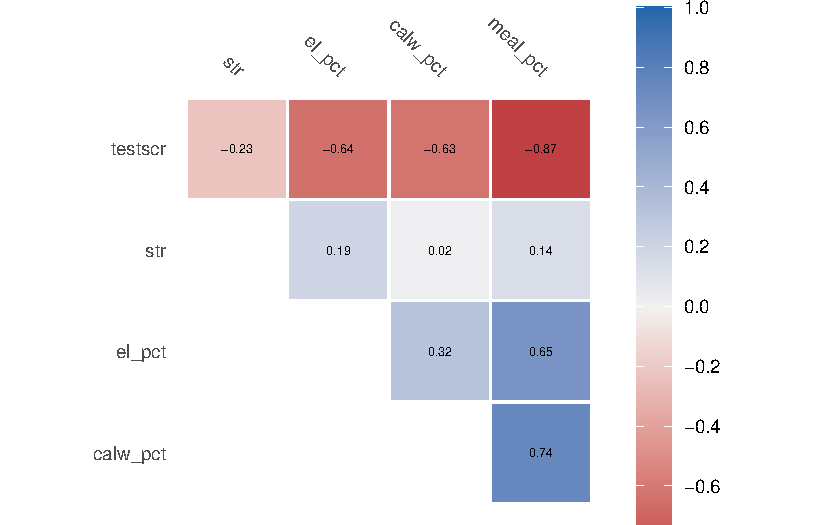
\includegraphics{Ch6_7_SW_files/figure-pdf/unnamed-chunk-8-1.pdf}

}

\end{figure}

\hypertarget{fig-7.2}{%
\subsection{Fig 7.2}\label{fig-7.2}}

\begin{Shaded}
\begin{Highlighting}[]
\NormalTok{p1}\OtherTok{\textless{}{-}} \FunctionTok{ggplot}\NormalTok{(caschool)}\SpecialCharTok{+}\FunctionTok{aes}\NormalTok{(}\AttributeTok{x=}\NormalTok{el\_pct,}\AttributeTok{y=}\NormalTok{testscr)}\SpecialCharTok{+}\FunctionTok{geom\_point}\NormalTok{()}\SpecialCharTok{+}
  \FunctionTok{labs}\NormalTok{(}\AttributeTok{x=}\StringTok{"percent"}\NormalTok{,}\AttributeTok{y=}\StringTok{"Test Score"}\NormalTok{)}
\NormalTok{p2}\OtherTok{\textless{}{-}} \FunctionTok{ggplot}\NormalTok{(caschool)}\SpecialCharTok{+}\FunctionTok{aes}\NormalTok{(}\AttributeTok{x=}\NormalTok{meal\_pct,}\AttributeTok{y=}\NormalTok{testscr)}\SpecialCharTok{+}\FunctionTok{geom\_point}\NormalTok{()}\SpecialCharTok{+}
  \FunctionTok{labs}\NormalTok{(}\AttributeTok{x=}\StringTok{"percent"}\NormalTok{,}\AttributeTok{y=}\StringTok{"Test Score"}\NormalTok{)}
\NormalTok{p3}\OtherTok{\textless{}{-}} \FunctionTok{ggplot}\NormalTok{(caschool)}\SpecialCharTok{+}\FunctionTok{aes}\NormalTok{(}\AttributeTok{x=}\NormalTok{calw\_pct,}\AttributeTok{y=}\NormalTok{testscr)}\SpecialCharTok{+}\FunctionTok{geom\_point}\NormalTok{()}\SpecialCharTok{+}
  \FunctionTok{labs}\NormalTok{(}\AttributeTok{x=}\StringTok{"percent"}\NormalTok{,}\AttributeTok{y=}\StringTok{"Test Score"}\NormalTok{)}
\FunctionTok{library}\NormalTok{(gridExtra)}
\end{Highlighting}
\end{Shaded}

\begin{verbatim}

Attaching package: 'gridExtra'
\end{verbatim}

\begin{verbatim}
The following object is masked from 'package:dplyr':

    combine
\end{verbatim}

\begin{Shaded}
\begin{Highlighting}[]
\CommentTok{\#grid.arrange(p1,p2,p3, nrow=3)}
\NormalTok{p1}
\end{Highlighting}
\end{Shaded}

\begin{figure}[H]

{\centering 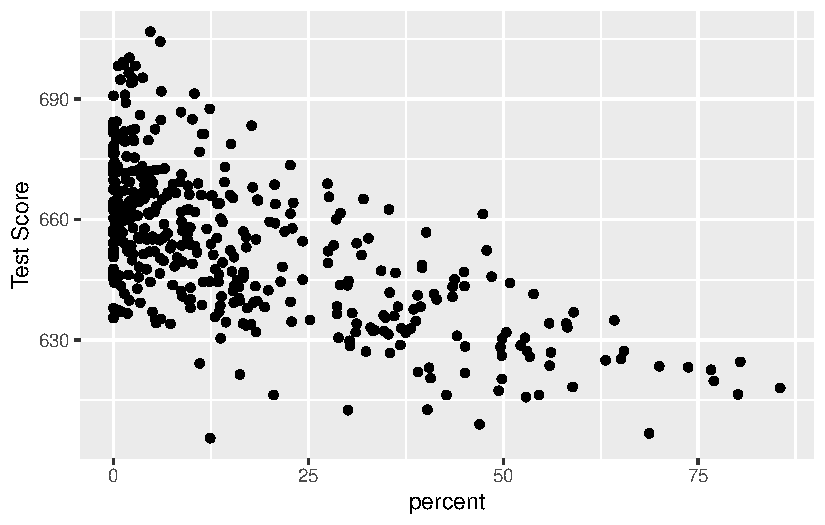
\includegraphics{Ch6_7_SW_files/figure-pdf/unnamed-chunk-9-1.pdf}

}

\end{figure}

\hypertarget{section-15}{%
\subsection{}\label{section-15}}

\begin{Shaded}
\begin{Highlighting}[]
\NormalTok{p2}
\end{Highlighting}
\end{Shaded}

\begin{figure}[H]

{\centering 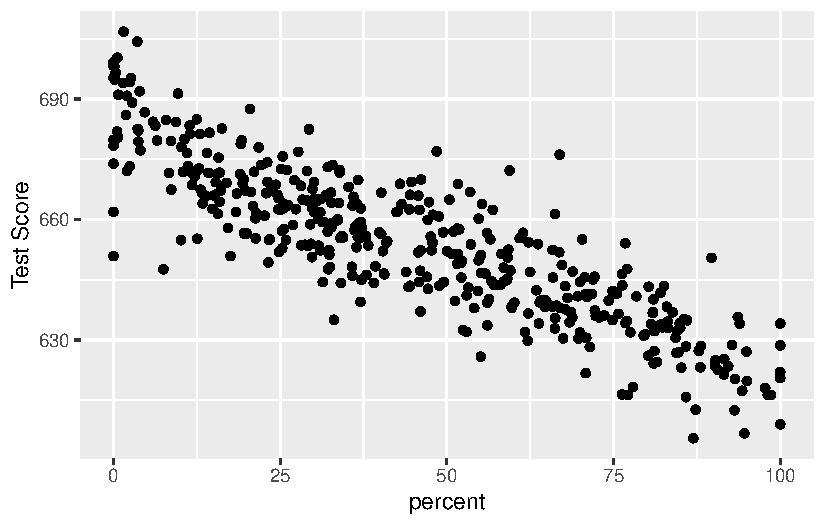
\includegraphics{Ch6_7_SW_files/figure-pdf/unnamed-chunk-10-1.pdf}

}

\end{figure}

\hypertarget{section-16}{%
\subsection{}\label{section-16}}

\begin{Shaded}
\begin{Highlighting}[]
\NormalTok{p3}
\end{Highlighting}
\end{Shaded}

\begin{figure}[H]

{\centering 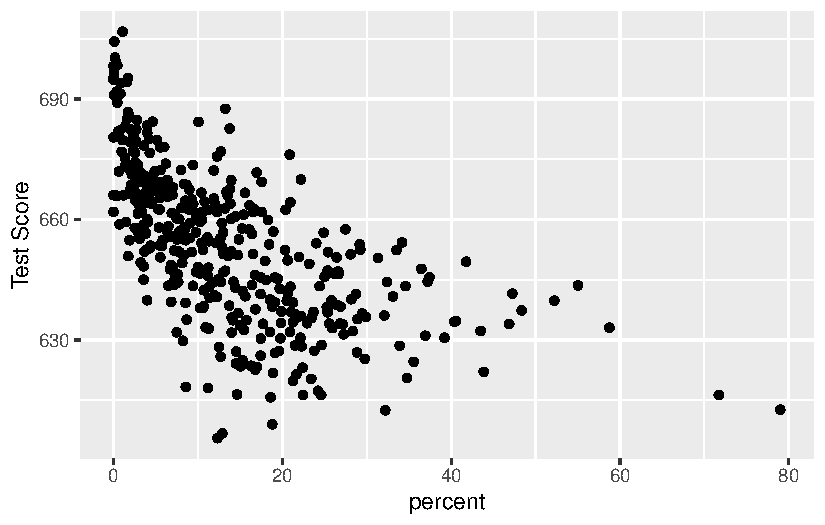
\includegraphics{Ch6_7_SW_files/figure-pdf/unnamed-chunk-11-1.pdf}

}

\end{figure}

\hypertarget{table-7.1-regressions-of-test-scores-on-student-teacher-ratio}{%
\subsection{Table 7.1 Regressions of Test Scores on Student-Teacher
Ratio}\label{table-7.1-regressions-of-test-scores-on-student-teacher-ratio}}

\begin{Shaded}
\begin{Highlighting}[]
\CommentTok{\#vtable(caschool)}
\NormalTok{m1}\OtherTok{\textless{}{-}}\FunctionTok{lm}\NormalTok{(testscr}\SpecialCharTok{\textasciitilde{}}\NormalTok{str,}\AttributeTok{data =}\NormalTok{ caschool)}
\NormalTok{m2}\OtherTok{\textless{}{-}}\FunctionTok{lm}\NormalTok{(testscr}\SpecialCharTok{\textasciitilde{}}\NormalTok{str}\SpecialCharTok{+}\NormalTok{el\_pct,}\AttributeTok{data =}\NormalTok{ caschool)}
\NormalTok{m3}\OtherTok{\textless{}{-}}\FunctionTok{lm}\NormalTok{(testscr}\SpecialCharTok{\textasciitilde{}}\NormalTok{str}\SpecialCharTok{+}\NormalTok{el\_pct}\SpecialCharTok{+}\NormalTok{meal\_pct,}\AttributeTok{data =}\NormalTok{ caschool)}
\NormalTok{m4}\OtherTok{\textless{}{-}}\FunctionTok{lm}\NormalTok{(testscr}\SpecialCharTok{\textasciitilde{}}\NormalTok{str}\SpecialCharTok{+}\NormalTok{el\_pct}\SpecialCharTok{+}\NormalTok{calw\_pct,}\AttributeTok{data =}\NormalTok{ caschool)}
\NormalTok{m5}\OtherTok{\textless{}{-}}\FunctionTok{lm}\NormalTok{(testscr}\SpecialCharTok{\textasciitilde{}}\NormalTok{str}\SpecialCharTok{+}\NormalTok{el\_pct}\SpecialCharTok{+}\NormalTok{meal\_pct}\SpecialCharTok{+}\NormalTok{calw\_pct,}\AttributeTok{data =}\NormalTok{ caschool)}
\FunctionTok{library}\NormalTok{(fixest)}
\FunctionTok{library}\NormalTok{(modelsummary)}
\NormalTok{models}\OtherTok{\textless{}{-}}\FunctionTok{list}\NormalTok{(m1,m2,m3,m4,m5)}
\FunctionTok{library}\NormalTok{(huxtable)}
\CommentTok{\#etable(m1,m2,m3,m4)}
\FunctionTok{modelsummary}\NormalTok{(models,}\AttributeTok{estimate =} \StringTok{"\{estimate\}\{stars\}"}\NormalTok{, }\AttributeTok{output=}\StringTok{"huxtable"}\NormalTok{)}
\end{Highlighting}
\end{Shaded}

 
  \providecommand{\huxb}[2]{\arrayrulecolor[RGB]{#1}\global\arrayrulewidth=#2pt}
  \providecommand{\huxvb}[2]{\color[RGB]{#1}\vrule width #2pt}
  \providecommand{\huxtpad}[1]{\rule{0pt}{#1}}
  \providecommand{\huxbpad}[1]{\rule[-#1]{0pt}{#1}}

\begin{table}[ht]
\begin{centerbox}
\begin{threeparttable}
 
\setlength{\tabcolsep}{0pt}
\begin{tabular}{l l l l l l}


\hhline{>{\huxb{0, 0, 0}{1}}->{\huxb{0, 0, 0}{1}}->{\huxb{0, 0, 0}{1}}->{\huxb{0, 0, 0}{1}}->{\huxb{0, 0, 0}{1}}->{\huxb{0, 0, 0}{1}}-}
\arrayrulecolor{black}

\multicolumn{1}{!{\huxvb{0, 0, 0}{0}}l!{\huxvb{0, 0, 0}{0}}}{\huxtpad{6pt + 1em}\raggedright \hspace{6pt}   \hspace{6pt}\huxbpad{6pt}} &
\multicolumn{1}{l!{\huxvb{0, 0, 0}{0}}}{\huxtpad{6pt + 1em}\raggedright \hspace{6pt} Model 1 \hspace{6pt}\huxbpad{6pt}} &
\multicolumn{1}{l!{\huxvb{0, 0, 0}{0}}}{\huxtpad{6pt + 1em}\raggedright \hspace{6pt} Model 2 \hspace{6pt}\huxbpad{6pt}} &
\multicolumn{1}{l!{\huxvb{0, 0, 0}{0}}}{\huxtpad{6pt + 1em}\raggedright \hspace{6pt} Model 3 \hspace{6pt}\huxbpad{6pt}} &
\multicolumn{1}{l!{\huxvb{0, 0, 0}{0}}}{\huxtpad{6pt + 1em}\raggedright \hspace{6pt} Model 4 \hspace{6pt}\huxbpad{6pt}} &
\multicolumn{1}{l!{\huxvb{0, 0, 0}{0}}}{\huxtpad{6pt + 1em}\raggedright \hspace{6pt} Model 5 \hspace{6pt}\huxbpad{6pt}} \tabularnewline[-0.5pt]


\hhline{>{\huxb{0, 0, 0}{1}}->{\huxb{0, 0, 0}{1}}->{\huxb{0, 0, 0}{1}}->{\huxb{0, 0, 0}{1}}->{\huxb{0, 0, 0}{1}}->{\huxb{0, 0, 0}{1}}-}
\arrayrulecolor{black}

\multicolumn{1}{!{\huxvb{0, 0, 0}{0}}l!{\huxvb{0, 0, 0}{0}}}{\huxtpad{6pt + 1em}\raggedright \hspace{6pt} (Intercept) \hspace{6pt}\huxbpad{6pt}} &
\multicolumn{1}{l!{\huxvb{0, 0, 0}{0}}}{\huxtpad{6pt + 1em}\raggedright \hspace{6pt} 698.933*** \hspace{6pt}\huxbpad{6pt}} &
\multicolumn{1}{l!{\huxvb{0, 0, 0}{0}}}{\huxtpad{6pt + 1em}\raggedright \hspace{6pt} 686.032*** \hspace{6pt}\huxbpad{6pt}} &
\multicolumn{1}{l!{\huxvb{0, 0, 0}{0}}}{\huxtpad{6pt + 1em}\raggedright \hspace{6pt} 700.150*** \hspace{6pt}\huxbpad{6pt}} &
\multicolumn{1}{l!{\huxvb{0, 0, 0}{0}}}{\huxtpad{6pt + 1em}\raggedright \hspace{6pt} 697.999*** \hspace{6pt}\huxbpad{6pt}} &
\multicolumn{1}{l!{\huxvb{0, 0, 0}{0}}}{\huxtpad{6pt + 1em}\raggedright \hspace{6pt} 700.392*** \hspace{6pt}\huxbpad{6pt}} \tabularnewline[-0.5pt]


\hhline{}
\arrayrulecolor{black}

\multicolumn{1}{!{\huxvb{0, 0, 0}{0}}l!{\huxvb{0, 0, 0}{0}}}{\huxtpad{6pt + 1em}\raggedright \hspace{6pt}  \hspace{6pt}\huxbpad{6pt}} &
\multicolumn{1}{l!{\huxvb{0, 0, 0}{0}}}{\huxtpad{6pt + 1em}\raggedright \hspace{6pt} (9.467) \hspace{6pt}\huxbpad{6pt}} &
\multicolumn{1}{l!{\huxvb{0, 0, 0}{0}}}{\huxtpad{6pt + 1em}\raggedright \hspace{6pt} (7.411) \hspace{6pt}\huxbpad{6pt}} &
\multicolumn{1}{l!{\huxvb{0, 0, 0}{0}}}{\huxtpad{6pt + 1em}\raggedright \hspace{6pt} (4.686) \hspace{6pt}\huxbpad{6pt}} &
\multicolumn{1}{l!{\huxvb{0, 0, 0}{0}}}{\huxtpad{6pt + 1em}\raggedright \hspace{6pt} (6.024) \hspace{6pt}\huxbpad{6pt}} &
\multicolumn{1}{l!{\huxvb{0, 0, 0}{0}}}{\huxtpad{6pt + 1em}\raggedright \hspace{6pt} (4.698) \hspace{6pt}\huxbpad{6pt}} \tabularnewline[-0.5pt]


\hhline{}
\arrayrulecolor{black}

\multicolumn{1}{!{\huxvb{0, 0, 0}{0}}l!{\huxvb{0, 0, 0}{0}}}{\huxtpad{6pt + 1em}\raggedright \hspace{6pt} str \hspace{6pt}\huxbpad{6pt}} &
\multicolumn{1}{l!{\huxvb{0, 0, 0}{0}}}{\huxtpad{6pt + 1em}\raggedright \hspace{6pt} -2.280*** \hspace{6pt}\huxbpad{6pt}} &
\multicolumn{1}{l!{\huxvb{0, 0, 0}{0}}}{\huxtpad{6pt + 1em}\raggedright \hspace{6pt} -1.101** \hspace{6pt}\huxbpad{6pt}} &
\multicolumn{1}{l!{\huxvb{0, 0, 0}{0}}}{\huxtpad{6pt + 1em}\raggedright \hspace{6pt} -0.998*** \hspace{6pt}\huxbpad{6pt}} &
\multicolumn{1}{l!{\huxvb{0, 0, 0}{0}}}{\huxtpad{6pt + 1em}\raggedright \hspace{6pt} -1.308*** \hspace{6pt}\huxbpad{6pt}} &
\multicolumn{1}{l!{\huxvb{0, 0, 0}{0}}}{\huxtpad{6pt + 1em}\raggedright \hspace{6pt} -1.014*** \hspace{6pt}\huxbpad{6pt}} \tabularnewline[-0.5pt]


\hhline{}
\arrayrulecolor{black}

\multicolumn{1}{!{\huxvb{0, 0, 0}{0}}l!{\huxvb{0, 0, 0}{0}}}{\huxtpad{6pt + 1em}\raggedright \hspace{6pt}  \hspace{6pt}\huxbpad{6pt}} &
\multicolumn{1}{l!{\huxvb{0, 0, 0}{0}}}{\huxtpad{6pt + 1em}\raggedright \hspace{6pt} (0.480) \hspace{6pt}\huxbpad{6pt}} &
\multicolumn{1}{l!{\huxvb{0, 0, 0}{0}}}{\huxtpad{6pt + 1em}\raggedright \hspace{6pt} (0.380) \hspace{6pt}\huxbpad{6pt}} &
\multicolumn{1}{l!{\huxvb{0, 0, 0}{0}}}{\huxtpad{6pt + 1em}\raggedright \hspace{6pt} (0.239) \hspace{6pt}\huxbpad{6pt}} &
\multicolumn{1}{l!{\huxvb{0, 0, 0}{0}}}{\huxtpad{6pt + 1em}\raggedright \hspace{6pt} (0.307) \hspace{6pt}\huxbpad{6pt}} &
\multicolumn{1}{l!{\huxvb{0, 0, 0}{0}}}{\huxtpad{6pt + 1em}\raggedright \hspace{6pt} (0.240) \hspace{6pt}\huxbpad{6pt}} \tabularnewline[-0.5pt]


\hhline{}
\arrayrulecolor{black}

\multicolumn{1}{!{\huxvb{0, 0, 0}{0}}l!{\huxvb{0, 0, 0}{0}}}{\huxtpad{6pt + 1em}\raggedright \hspace{6pt} el\_pct \hspace{6pt}\huxbpad{6pt}} &
\multicolumn{1}{l!{\huxvb{0, 0, 0}{0}}}{\huxtpad{6pt + 1em}\raggedright \hspace{6pt}  \hspace{6pt}\huxbpad{6pt}} &
\multicolumn{1}{l!{\huxvb{0, 0, 0}{0}}}{\huxtpad{6pt + 1em}\raggedright \hspace{6pt} -0.650*** \hspace{6pt}\huxbpad{6pt}} &
\multicolumn{1}{l!{\huxvb{0, 0, 0}{0}}}{\huxtpad{6pt + 1em}\raggedright \hspace{6pt} -0.122*** \hspace{6pt}\huxbpad{6pt}} &
\multicolumn{1}{l!{\huxvb{0, 0, 0}{0}}}{\huxtpad{6pt + 1em}\raggedright \hspace{6pt} -0.488*** \hspace{6pt}\huxbpad{6pt}} &
\multicolumn{1}{l!{\huxvb{0, 0, 0}{0}}}{\huxtpad{6pt + 1em}\raggedright \hspace{6pt} -0.130*** \hspace{6pt}\huxbpad{6pt}} \tabularnewline[-0.5pt]


\hhline{}
\arrayrulecolor{black}

\multicolumn{1}{!{\huxvb{0, 0, 0}{0}}l!{\huxvb{0, 0, 0}{0}}}{\huxtpad{6pt + 1em}\raggedright \hspace{6pt}  \hspace{6pt}\huxbpad{6pt}} &
\multicolumn{1}{l!{\huxvb{0, 0, 0}{0}}}{\huxtpad{6pt + 1em}\raggedright \hspace{6pt}  \hspace{6pt}\huxbpad{6pt}} &
\multicolumn{1}{l!{\huxvb{0, 0, 0}{0}}}{\huxtpad{6pt + 1em}\raggedright \hspace{6pt} (0.039) \hspace{6pt}\huxbpad{6pt}} &
\multicolumn{1}{l!{\huxvb{0, 0, 0}{0}}}{\huxtpad{6pt + 1em}\raggedright \hspace{6pt} (0.032) \hspace{6pt}\huxbpad{6pt}} &
\multicolumn{1}{l!{\huxvb{0, 0, 0}{0}}}{\huxtpad{6pt + 1em}\raggedright \hspace{6pt} (0.033) \hspace{6pt}\huxbpad{6pt}} &
\multicolumn{1}{l!{\huxvb{0, 0, 0}{0}}}{\huxtpad{6pt + 1em}\raggedright \hspace{6pt} (0.034) \hspace{6pt}\huxbpad{6pt}} \tabularnewline[-0.5pt]


\hhline{}
\arrayrulecolor{black}

\multicolumn{1}{!{\huxvb{0, 0, 0}{0}}l!{\huxvb{0, 0, 0}{0}}}{\huxtpad{6pt + 1em}\raggedright \hspace{6pt} meal\_pct \hspace{6pt}\huxbpad{6pt}} &
\multicolumn{1}{l!{\huxvb{0, 0, 0}{0}}}{\huxtpad{6pt + 1em}\raggedright \hspace{6pt}  \hspace{6pt}\huxbpad{6pt}} &
\multicolumn{1}{l!{\huxvb{0, 0, 0}{0}}}{\huxtpad{6pt + 1em}\raggedright \hspace{6pt}  \hspace{6pt}\huxbpad{6pt}} &
\multicolumn{1}{l!{\huxvb{0, 0, 0}{0}}}{\huxtpad{6pt + 1em}\raggedright \hspace{6pt} -0.547*** \hspace{6pt}\huxbpad{6pt}} &
\multicolumn{1}{l!{\huxvb{0, 0, 0}{0}}}{\huxtpad{6pt + 1em}\raggedright \hspace{6pt}  \hspace{6pt}\huxbpad{6pt}} &
\multicolumn{1}{l!{\huxvb{0, 0, 0}{0}}}{\huxtpad{6pt + 1em}\raggedright \hspace{6pt} -0.529*** \hspace{6pt}\huxbpad{6pt}} \tabularnewline[-0.5pt]


\hhline{}
\arrayrulecolor{black}

\multicolumn{1}{!{\huxvb{0, 0, 0}{0}}l!{\huxvb{0, 0, 0}{0}}}{\huxtpad{6pt + 1em}\raggedright \hspace{6pt}  \hspace{6pt}\huxbpad{6pt}} &
\multicolumn{1}{l!{\huxvb{0, 0, 0}{0}}}{\huxtpad{6pt + 1em}\raggedright \hspace{6pt}  \hspace{6pt}\huxbpad{6pt}} &
\multicolumn{1}{l!{\huxvb{0, 0, 0}{0}}}{\huxtpad{6pt + 1em}\raggedright \hspace{6pt}  \hspace{6pt}\huxbpad{6pt}} &
\multicolumn{1}{l!{\huxvb{0, 0, 0}{0}}}{\huxtpad{6pt + 1em}\raggedright \hspace{6pt} (0.022) \hspace{6pt}\huxbpad{6pt}} &
\multicolumn{1}{l!{\huxvb{0, 0, 0}{0}}}{\huxtpad{6pt + 1em}\raggedright \hspace{6pt}  \hspace{6pt}\huxbpad{6pt}} &
\multicolumn{1}{l!{\huxvb{0, 0, 0}{0}}}{\huxtpad{6pt + 1em}\raggedright \hspace{6pt} (0.032) \hspace{6pt}\huxbpad{6pt}} \tabularnewline[-0.5pt]


\hhline{}
\arrayrulecolor{black}

\multicolumn{1}{!{\huxvb{0, 0, 0}{0}}l!{\huxvb{0, 0, 0}{0}}}{\huxtpad{6pt + 1em}\raggedright \hspace{6pt} calw\_pct \hspace{6pt}\huxbpad{6pt}} &
\multicolumn{1}{l!{\huxvb{0, 0, 0}{0}}}{\huxtpad{6pt + 1em}\raggedright \hspace{6pt}  \hspace{6pt}\huxbpad{6pt}} &
\multicolumn{1}{l!{\huxvb{0, 0, 0}{0}}}{\huxtpad{6pt + 1em}\raggedright \hspace{6pt}  \hspace{6pt}\huxbpad{6pt}} &
\multicolumn{1}{l!{\huxvb{0, 0, 0}{0}}}{\huxtpad{6pt + 1em}\raggedright \hspace{6pt}  \hspace{6pt}\huxbpad{6pt}} &
\multicolumn{1}{l!{\huxvb{0, 0, 0}{0}}}{\huxtpad{6pt + 1em}\raggedright \hspace{6pt} -0.790*** \hspace{6pt}\huxbpad{6pt}} &
\multicolumn{1}{l!{\huxvb{0, 0, 0}{0}}}{\huxtpad{6pt + 1em}\raggedright \hspace{6pt} -0.048 \hspace{6pt}\huxbpad{6pt}} \tabularnewline[-0.5pt]


\hhline{}
\arrayrulecolor{black}

\multicolumn{1}{!{\huxvb{0, 0, 0}{0}}l!{\huxvb{0, 0, 0}{0}}}{\huxtpad{6pt + 1em}\raggedright \hspace{6pt}  \hspace{6pt}\huxbpad{6pt}} &
\multicolumn{1}{l!{\huxvb{0, 0, 0}{0}}}{\huxtpad{6pt + 1em}\raggedright \hspace{6pt}  \hspace{6pt}\huxbpad{6pt}} &
\multicolumn{1}{l!{\huxvb{0, 0, 0}{0}}}{\huxtpad{6pt + 1em}\raggedright \hspace{6pt}  \hspace{6pt}\huxbpad{6pt}} &
\multicolumn{1}{l!{\huxvb{0, 0, 0}{0}}}{\huxtpad{6pt + 1em}\raggedright \hspace{6pt}  \hspace{6pt}\huxbpad{6pt}} &
\multicolumn{1}{l!{\huxvb{0, 0, 0}{0}}}{\huxtpad{6pt + 1em}\raggedright \hspace{6pt} (0.053) \hspace{6pt}\huxbpad{6pt}} &
\multicolumn{1}{l!{\huxvb{0, 0, 0}{0}}}{\huxtpad{6pt + 1em}\raggedright \hspace{6pt} (0.061) \hspace{6pt}\huxbpad{6pt}} \tabularnewline[-0.5pt]


\hhline{>{\huxb{0, 0, 0}{1}}->{\huxb{0, 0, 0}{1}}->{\huxb{0, 0, 0}{1}}->{\huxb{0, 0, 0}{1}}->{\huxb{0, 0, 0}{1}}->{\huxb{0, 0, 0}{1}}-}
\arrayrulecolor{black}

\multicolumn{1}{!{\huxvb{0, 0, 0}{0}}l!{\huxvb{0, 0, 0}{0}}}{\huxtpad{6pt + 1em}\raggedright \hspace{6pt} Num.Obs. \hspace{6pt}\huxbpad{6pt}} &
\multicolumn{1}{l!{\huxvb{0, 0, 0}{0}}}{\huxtpad{6pt + 1em}\raggedright \hspace{6pt} 420 \hspace{6pt}\huxbpad{6pt}} &
\multicolumn{1}{l!{\huxvb{0, 0, 0}{0}}}{\huxtpad{6pt + 1em}\raggedright \hspace{6pt} 420 \hspace{6pt}\huxbpad{6pt}} &
\multicolumn{1}{l!{\huxvb{0, 0, 0}{0}}}{\huxtpad{6pt + 1em}\raggedright \hspace{6pt} 420 \hspace{6pt}\huxbpad{6pt}} &
\multicolumn{1}{l!{\huxvb{0, 0, 0}{0}}}{\huxtpad{6pt + 1em}\raggedright \hspace{6pt} 420 \hspace{6pt}\huxbpad{6pt}} &
\multicolumn{1}{l!{\huxvb{0, 0, 0}{0}}}{\huxtpad{6pt + 1em}\raggedright \hspace{6pt} 420 \hspace{6pt}\huxbpad{6pt}} \tabularnewline[-0.5pt]


\hhline{}
\arrayrulecolor{black}

\multicolumn{1}{!{\huxvb{0, 0, 0}{0}}l!{\huxvb{0, 0, 0}{0}}}{\huxtpad{6pt + 1em}\raggedright \hspace{6pt} R2 \hspace{6pt}\huxbpad{6pt}} &
\multicolumn{1}{l!{\huxvb{0, 0, 0}{0}}}{\huxtpad{6pt + 1em}\raggedright \hspace{6pt} 0.051 \hspace{6pt}\huxbpad{6pt}} &
\multicolumn{1}{l!{\huxvb{0, 0, 0}{0}}}{\huxtpad{6pt + 1em}\raggedright \hspace{6pt} 0.426 \hspace{6pt}\huxbpad{6pt}} &
\multicolumn{1}{l!{\huxvb{0, 0, 0}{0}}}{\huxtpad{6pt + 1em}\raggedright \hspace{6pt} 0.775 \hspace{6pt}\huxbpad{6pt}} &
\multicolumn{1}{l!{\huxvb{0, 0, 0}{0}}}{\huxtpad{6pt + 1em}\raggedright \hspace{6pt} 0.629 \hspace{6pt}\huxbpad{6pt}} &
\multicolumn{1}{l!{\huxvb{0, 0, 0}{0}}}{\huxtpad{6pt + 1em}\raggedright \hspace{6pt} 0.775 \hspace{6pt}\huxbpad{6pt}} \tabularnewline[-0.5pt]


\hhline{}
\arrayrulecolor{black}

\multicolumn{1}{!{\huxvb{0, 0, 0}{0}}l!{\huxvb{0, 0, 0}{0}}}{\huxtpad{6pt + 1em}\raggedright \hspace{6pt} R2 Adj. \hspace{6pt}\huxbpad{6pt}} &
\multicolumn{1}{l!{\huxvb{0, 0, 0}{0}}}{\huxtpad{6pt + 1em}\raggedright \hspace{6pt} 0.049 \hspace{6pt}\huxbpad{6pt}} &
\multicolumn{1}{l!{\huxvb{0, 0, 0}{0}}}{\huxtpad{6pt + 1em}\raggedright \hspace{6pt} 0.424 \hspace{6pt}\huxbpad{6pt}} &
\multicolumn{1}{l!{\huxvb{0, 0, 0}{0}}}{\huxtpad{6pt + 1em}\raggedright \hspace{6pt} 0.773 \hspace{6pt}\huxbpad{6pt}} &
\multicolumn{1}{l!{\huxvb{0, 0, 0}{0}}}{\huxtpad{6pt + 1em}\raggedright \hspace{6pt} 0.626 \hspace{6pt}\huxbpad{6pt}} &
\multicolumn{1}{l!{\huxvb{0, 0, 0}{0}}}{\huxtpad{6pt + 1em}\raggedright \hspace{6pt} 0.773 \hspace{6pt}\huxbpad{6pt}} \tabularnewline[-0.5pt]


\hhline{}
\arrayrulecolor{black}

\multicolumn{1}{!{\huxvb{0, 0, 0}{0}}l!{\huxvb{0, 0, 0}{0}}}{\huxtpad{6pt + 1em}\raggedright \hspace{6pt} AIC \hspace{6pt}\huxbpad{6pt}} &
\multicolumn{1}{l!{\huxvb{0, 0, 0}{0}}}{\huxtpad{6pt + 1em}\raggedright \hspace{6pt} 3650.5 \hspace{6pt}\huxbpad{6pt}} &
\multicolumn{1}{l!{\huxvb{0, 0, 0}{0}}}{\huxtpad{6pt + 1em}\raggedright \hspace{6pt} 3441.1 \hspace{6pt}\huxbpad{6pt}} &
\multicolumn{1}{l!{\huxvb{0, 0, 0}{0}}}{\huxtpad{6pt + 1em}\raggedright \hspace{6pt} 3051.0 \hspace{6pt}\huxbpad{6pt}} &
\multicolumn{1}{l!{\huxvb{0, 0, 0}{0}}}{\huxtpad{6pt + 1em}\raggedright \hspace{6pt} 3260.7 \hspace{6pt}\huxbpad{6pt}} &
\multicolumn{1}{l!{\huxvb{0, 0, 0}{0}}}{\huxtpad{6pt + 1em}\raggedright \hspace{6pt} 3052.4 \hspace{6pt}\huxbpad{6pt}} \tabularnewline[-0.5pt]


\hhline{}
\arrayrulecolor{black}

\multicolumn{1}{!{\huxvb{0, 0, 0}{0}}l!{\huxvb{0, 0, 0}{0}}}{\huxtpad{6pt + 1em}\raggedright \hspace{6pt} BIC \hspace{6pt}\huxbpad{6pt}} &
\multicolumn{1}{l!{\huxvb{0, 0, 0}{0}}}{\huxtpad{6pt + 1em}\raggedright \hspace{6pt} 3662.6 \hspace{6pt}\huxbpad{6pt}} &
\multicolumn{1}{l!{\huxvb{0, 0, 0}{0}}}{\huxtpad{6pt + 1em}\raggedright \hspace{6pt} 3457.3 \hspace{6pt}\huxbpad{6pt}} &
\multicolumn{1}{l!{\huxvb{0, 0, 0}{0}}}{\huxtpad{6pt + 1em}\raggedright \hspace{6pt} 3071.2 \hspace{6pt}\huxbpad{6pt}} &
\multicolumn{1}{l!{\huxvb{0, 0, 0}{0}}}{\huxtpad{6pt + 1em}\raggedright \hspace{6pt} 3280.9 \hspace{6pt}\huxbpad{6pt}} &
\multicolumn{1}{l!{\huxvb{0, 0, 0}{0}}}{\huxtpad{6pt + 1em}\raggedright \hspace{6pt} 3076.6 \hspace{6pt}\huxbpad{6pt}} \tabularnewline[-0.5pt]


\hhline{}
\arrayrulecolor{black}

\multicolumn{1}{!{\huxvb{0, 0, 0}{0}}l!{\huxvb{0, 0, 0}{0}}}{\huxtpad{6pt + 1em}\raggedright \hspace{6pt} Log.Lik. \hspace{6pt}\huxbpad{6pt}} &
\multicolumn{1}{l!{\huxvb{0, 0, 0}{0}}}{\huxtpad{6pt + 1em}\raggedright \hspace{6pt} -1822.250 \hspace{6pt}\huxbpad{6pt}} &
\multicolumn{1}{l!{\huxvb{0, 0, 0}{0}}}{\huxtpad{6pt + 1em}\raggedright \hspace{6pt} -1716.561 \hspace{6pt}\huxbpad{6pt}} &
\multicolumn{1}{l!{\huxvb{0, 0, 0}{0}}}{\huxtpad{6pt + 1em}\raggedright \hspace{6pt} -1520.499 \hspace{6pt}\huxbpad{6pt}} &
\multicolumn{1}{l!{\huxvb{0, 0, 0}{0}}}{\huxtpad{6pt + 1em}\raggedright \hspace{6pt} -1625.328 \hspace{6pt}\huxbpad{6pt}} &
\multicolumn{1}{l!{\huxvb{0, 0, 0}{0}}}{\huxtpad{6pt + 1em}\raggedright \hspace{6pt} -1520.188 \hspace{6pt}\huxbpad{6pt}} \tabularnewline[-0.5pt]


\hhline{}
\arrayrulecolor{black}

\multicolumn{1}{!{\huxvb{0, 0, 0}{0}}l!{\huxvb{0, 0, 0}{0}}}{\huxtpad{6pt + 1em}\raggedright \hspace{6pt} F \hspace{6pt}\huxbpad{6pt}} &
\multicolumn{1}{l!{\huxvb{0, 0, 0}{0}}}{\huxtpad{6pt + 1em}\raggedright \hspace{6pt} 22.575 \hspace{6pt}\huxbpad{6pt}} &
\multicolumn{1}{l!{\huxvb{0, 0, 0}{0}}}{\huxtpad{6pt + 1em}\raggedright \hspace{6pt} 155.014 \hspace{6pt}\huxbpad{6pt}} &
\multicolumn{1}{l!{\huxvb{0, 0, 0}{0}}}{\huxtpad{6pt + 1em}\raggedright \hspace{6pt} 476.306 \hspace{6pt}\huxbpad{6pt}} &
\multicolumn{1}{l!{\huxvb{0, 0, 0}{0}}}{\huxtpad{6pt + 1em}\raggedright \hspace{6pt} 234.638 \hspace{6pt}\huxbpad{6pt}} &
\multicolumn{1}{l!{\huxvb{0, 0, 0}{0}}}{\huxtpad{6pt + 1em}\raggedright \hspace{6pt} 357.054 \hspace{6pt}\huxbpad{6pt}} \tabularnewline[-0.5pt]


\hhline{}
\arrayrulecolor{black}

\multicolumn{1}{!{\huxvb{0, 0, 0}{0}}l!{\huxvb{0, 0, 0}{0}}}{\huxtpad{6pt + 1em}\raggedright \hspace{6pt} RMSE \hspace{6pt}\huxbpad{6pt}} &
\multicolumn{1}{l!{\huxvb{0, 0, 0}{0}}}{\huxtpad{6pt + 1em}\raggedright \hspace{6pt} 18.54 \hspace{6pt}\huxbpad{6pt}} &
\multicolumn{1}{l!{\huxvb{0, 0, 0}{0}}}{\huxtpad{6pt + 1em}\raggedright \hspace{6pt} 14.41 \hspace{6pt}\huxbpad{6pt}} &
\multicolumn{1}{l!{\huxvb{0, 0, 0}{0}}}{\huxtpad{6pt + 1em}\raggedright \hspace{6pt} 9.04 \hspace{6pt}\huxbpad{6pt}} &
\multicolumn{1}{l!{\huxvb{0, 0, 0}{0}}}{\huxtpad{6pt + 1em}\raggedright \hspace{6pt} 11.60 \hspace{6pt}\huxbpad{6pt}} &
\multicolumn{1}{l!{\huxvb{0, 0, 0}{0}}}{\huxtpad{6pt + 1em}\raggedright \hspace{6pt} 9.03 \hspace{6pt}\huxbpad{6pt}} \tabularnewline[-0.5pt]


\hhline{>{\huxb{0, 0, 0}{1}}->{\huxb{0, 0, 0}{1}}->{\huxb{0, 0, 0}{1}}->{\huxb{0, 0, 0}{1}}->{\huxb{0, 0, 0}{1}}->{\huxb{0, 0, 0}{1}}-}
\arrayrulecolor{black}
\end{tabular}
\end{threeparttable}\par\end{centerbox}

\end{table}
 

\begin{Shaded}
\begin{Highlighting}[]
\CommentTok{\#modelsummary(models, fmt=4)}
\CommentTok{\#modelsummary(models,}
 \CommentTok{\#            statistic = "\{std.error\} (\{p.value\})")}
\CommentTok{\#modelsummary(models,}
 \CommentTok{\#            estimate = "\{estimate\}\{stars\}",}
  \CommentTok{\#           gof\_omit = ".*")}
\end{Highlighting}
\end{Shaded}




\end{document}
